\begin{center}
\Huge
Funktionstyper 
\end{center}
\section*{Sammensatte funktioner}
\stepcounter{section}
En sammensat funktion er - som navnet hentyder til - funktioner, der er sat sammen. Mere præcist har vi en definition.
\begin{defn}
Har vi to funktioner $f$ og $g$, så kan vi bestemme  den sammensatte funktion af $f$ og $g$ som
\begin{align*}
f(g(x)).
\end{align*}
Dette skrives også til tider $f(g(x))= g\circ f(x)$. I dette tilfælde kaldes $g$ for den indre funktion og $f$ for den ydre funktion.
\end{defn}
\begin{exa}
Lad $f$ og $g$ være givet ved henholdsvist
\begin{align*}
f(x) = \sqrt{x} \textnormal{ og }g(x) = 3\cdot x.
\end{align*}
Så er den sammensatte funktion $f(g(x))$ bestemt ved
\begin{align*}
f(g(x)) = \sqrt{3\cdot x}.
\end{align*}
Tilsvarende er den sammensatte funktion $g(f(x))$ bestemt ved
\begin{align*}
g(f(x)) = 3\sqrt{x}.
\end{align*}
\end{exa}
\begin{exa}
CO$_2$-koncentrationen i en beholder kan tilnærmes ved $f(x) = 10\cdot x+385$, hvor $f$ er i ppm (parts per million) og $x$ er antallet af en bestemt type bakterier i mio. Antallet af bakterier (i mio.) i beholderen kan i et begrænset tidsinterval beskrives ved $g(t)= 2\cdot 1.07^t$, hvor $t$ beskriver tiden i timer. CO$_2$-koncentrationen som funktion af tid kan derfor beskrives ved
\begin{align*}
f(g(t)) = 10\cdot (2\cdot 1.07^t) + 385 = 20\cdot 1.07^t + 385.
\end{align*}
\section*{Stykvist definerede funktioner}
\stepcounter{section}
En stykvist defineret funktion er en funktion, der er defineret på forskellige måder alt efter hvad $x$ er.
\begin{exa}
Et taxafirma tager følgende pris for taxakørsel: De første to kilometer koster 10kr pr kilometer, de næste 5km koster 7 kr pr kilometer, og resten at afstanden koster taxaen 5kr pr kilometer. Vi kan definere prisen $p(x)$ som en stykvist defineret funktion:
\begin{align*}
p(x)=
\begin{cases}
10\cdot x, \ &0\leq x \leq 2,\\
7\cdot x + 6,\ &2 < x \leq 7,\\
5 \cdot x + 20,\ &7<x,
\end{cases}
\end{align*}
hvor $x$ er antal kilometer kørt og $p(x)$ er prisen i kr. 
\end{exa}
Grafen for $p$ kan ses på Fig. \ref{fig:stykvis}
\begin{figure}[H]
\centering
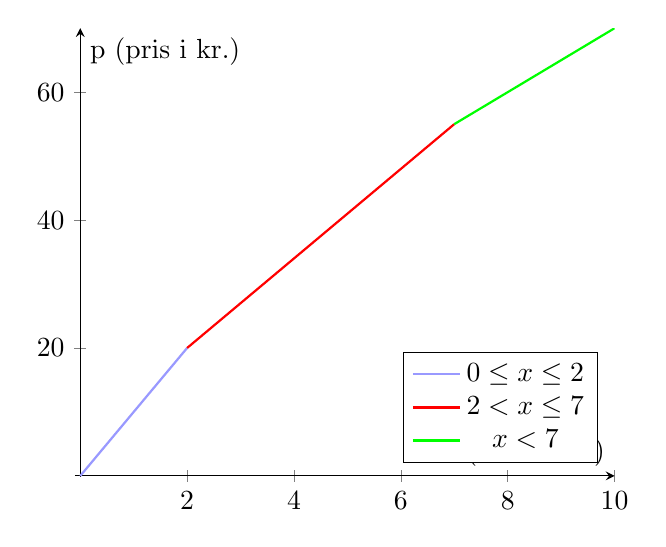
\begin{tikzpicture}
\begin{axis}[axis lines=middle, xmin = -0.1,ymin=-0.1,
legend pos = south east, 
xlabel={x (kørte km.)},
ylabel = {p (pris i kr.)}
]
\addplot[color=blue!40,samples = 1000, thick, domain = 0:2] {10*x};
\addplot[color=red,samples = 1000,thick,domain=2:7] {7*x+6};
\addplot[color=green,samples = 1000,thick,domain=7:10] {5*x+20};
\legend{$0\leq x \leq 2$,$2<x\leq 7$,$x<7$}
\end{axis}
\end{tikzpicture}
\caption{Pris for taxa som funktion af kørte km.}
\label{fig:stykvis}
\end{figure}
\end{exa}
\section*{Definitionsmængde og værdimængde}
\stepcounter{section}
Når vi har med funktioner at gøre, så er det altid implicit, hvilke værdier vi kan vælge som $x$-værdier. Skal man være mere præcis, så skal vi, når vi introducerer funktioner, altid fortælle, hvad vi må vælge $x$ til at være, samt hvad $f(x)$ kan være. 
\begin{defn}[Definitionsmængde]
\textit{Definitionsmængden} for en funktion $f$, er den mængde, funktionen afbilder fra. Den består altså at de tal, vi må vælge $x$ til at være i funktionsudtrykket $f(x)$. Vi skriver til tider Dm$(f)$ for definitionsmængden. Definitionsmængden kaldes også for domænet.
\end{defn}
\begin{defn}[Værdimængde]
\textit{Værdimængden} for en funktion $f$ er den mængde, funktionen afbilder over i. Vi skriver til tider Vm$(f)$ for værdimængden. Værdimængden kaldes også for billedmængden.
\end{defn}
\begin{exa}
For funktionen $f(x) = 2x$ er Vm$(f) = \textnormal{Dm}(f) = \mathbb{R}$. Vi kan stoppe alle tal ind på $x$, og funktionen giver os reelle tal.  
\end{exa}
\begin{exa}
Funktionen $g(x) = x^2$ har $\textnormal{Dm}(g) = \mathbb{R}$, men $\textnormal{Vm}(g) = \mathbb{R}_{\geq 0}$, altså kun de ikke-negative tal.
\end{exa}
Vi husker på, at potensfunktioner kun var defineret i første kvadrant. Der gælder derfor for potensfunktioner $f$, at $\textnormal{Dm}(f) = \textnormal{Vm}(f) = \mathbb{R}_{\geq 0}$. Hvis vi mere eksplicit vil opskrive, hvad værdimængden og definitionsmængden for en funktion er, så skriver vi $f: \textnormal{Dm}(f) \to \textnormal{Vm}(f)$. Eksempelvis har vi, $f:\mathbb{R} \to \mathbb{R}$ givet ved 
\begin{align*}
f(x) = x^3.
\end{align*}
\section*{Opgave 1}
For følgende funktioner $f$ og $g$, bestem så den sammensatte funktion $f(g(x))$ og $g(f(g))$.
\begin{align*}
&f(x) = \sqrt{x}\  \textnormal{ og } g(x) = x^2\\
&f(x) = 2x^3\  \textnormal{ og } g(x) = 10x+3\\
&f(x) = \ln(x)\  \textnormal{ og } g(x) = \frac{1}{x}\\
&f(x) = \sqrt[10]{x}\  \textnormal{ og } g(x) = x^{20}
\end{align*}
\section*{Opgave 2}
For $f(x) = x^2$ og $g(x)=2x+3$ løs ligningen
\begin{align*}
f(g(x)) = 0.
\end{align*}
\section*{Opgave 3}
En funktion $f$ er bestemt ved $\sqrt{x}$ for $x\geq 0$ og $x^2$ for $x<0$. Hvad er $f(2)$ og $f(-2)$?. Prøv at tegne $f$. 
\section*{Opgave 4}
Bestem definitionsmængde og værdimængde for følgende funktioner
\begin{align*}
&1) \ x  &&2) \ \sqrt{x}  \\
&3) \ 10x^3  &&4) \ \ln(x)  \\
&5) \  \ln(x^2) &&6) \ x^4   \\
\end{align*}
\section*{Opgave 5}
Funktionen $f(x) = \lceil x \rceil$ runder $x$ op til nærmeste heltal. Hvad er værdimængden og definitionsmængden for $f$?